\RequirePackage{currfile} 
\documentclass{beamer}
\usetheme{Edinburgh}
%%%%%%%%%%%%%%%%%%%%%%%%%%%%%%%%%%%%%%%%%
% Beamer Presentation
% LaTeX Template
% Version 1.0 (10/11/12)
%
% This template has been downloaded from:
% http://www.LaTeXTemplates.com
%
% License:
% CC BY-NC-SA 3.0 (http://creativecommons.org/licenses/by-nc-sa/3.0/)
%
%%%%%%%%%%%%%%%%%%%%%%%%%%%%%%%%%%%%%%%%%

%----------------------------------------------------------------------------------------
%	PACKAGES AND THEMES
%----------------------------------------------------------------------------------------




\mode<presentation> {

% The Beamer class comes with a number of default slide themes
% which change the colors and layouts of slides. Below this is a list
% of all the themes, uncomment each in turn to see what they look like.

%\usetheme{default}
%\usetheme{AnnArbor}
%\usetheme{Antibes}
%\usetheme{Bergen}
%\usetheme{Berkeley}
%\usetheme{Berlin}
%\usetheme{Boadilla}
%\usetheme{CambridgeUS}
%\usetheme{Copenhagen}
%\usetheme{Darmstadt}
%\usetheme{Dresden}
%\usetheme{Frankfurt}
%\usetheme{Goettingen}
%\usetheme{Hannover}
%\usetheme{Ilmenau}
%\usetheme{JuanLesPins}
%\usetheme{Luebeck}
%\usetheme{Madrid}		
%\usetheme{Malmoe}
%\usetheme{Marburg}
%\usetheme{Montpellier}
%\usetheme{PaloAlto}
%\usetheme{Pittsburgh}
%\usetheme{Rochester}
%\usetheme{Singapore}
%\usetheme{Szeged}
\usetheme{Warsaw}

% As well as themes, the Beamer class has a number of color themes
% for any slide theme. Uncomment each of these in turn to see how it
% changes the colors of your current slide theme.

%\usecolortheme{albatross}
%\usecolortheme{beaver}
%\usecolortheme{beetle}
%\usecolortheme{crane}
%\usecolortheme{dolphin}
%\usecolortheme{dove}
%\usecolortheme{fly}
%\usecolortheme{lily}
%\usecolortheme{orchid}
%\usecolortheme{rose}
%\usecolortheme{seagull}
%\usecolortheme{seahorse}
\usecolortheme{whale}
%\usecolortheme{wolverine}

%\setbeamertemplate{footline} % To remove the footer line in all slides uncomment this line
%\setbeamertemplate{footline}[frame number] % To replace the footer line in all slides with a simple slide count uncomment this line

%\setbeamertemplate{navigation symbols}{} % To remove the navigation symbols from the bottom of all slides uncomment this line

\setbeamercovered{transparent} % Fait apparaître les animations en grisé (utile pour la conception, mais peut être commenté lors de la remise du document final)

% Pour utiliser une police à empattements partout
\usefonttheme{serif}

% Pour rajouter la numérotation des frames dans les pieds de page
\newcommand*\oldmacro{}%
\let\oldmacro\insertshorttitle%
\renewcommand*\insertshorttitle{%
  \oldmacro\hfill%
  \insertframenumber\,/\,\inserttotalframenumber}

}

\usepackage{graphicx} % Allows including images
\usepackage{booktabs} % Allows the use of \toprule, \midrule and \bottomrule in tables



%
% XeTeX specific
%
\RequireXeTeX
\usepackage{xltxtra}
\usepackage{fontspec}
\usepackage{xunicode}

% -----------------------------------
% font config
% -----------------------------------

\setsansfont{Linux Biolinum}
\setromanfont{Linux Libertine}
\setmonofont[Scale=0.9]{Consolas}

% -----------------------------------
% math
% -----------------------------------

\usepackage{amsmath}
\usepackage{amsfonts}
\usepackage{amssymb}
\usepackage{amsthm}
\usepackage{mathrsfs}   % \mathscr
\usepackage{stmaryrd}   % \lightning

% -----------------------------------
% grammar and textstyle
% -----------------------------------

\usepackage{polyglossia}
\setdefaultlanguage[variant=british]{english}
\usepackage{csquotes}
% underlining
\usepackage{soul} % ulem redifines \emph, this sucks

% -----------------------------------
% colors
% -----------------------------------

\usepackage{xcolor}
\usepackage{colortbl}

% listing colors
% https://kuler.adobe.com/Color-palette-color-theme-4004722
\definecolor{keyword}{RGB}{239,33,74}
\definecolor{number}{RGB}{243,202,22}
\definecolor{comment}{RGB}{126,158,19}
\definecolor{string}{RGB}{6,129,128}


% -----------------------------------
% links and references
% -----------------------------------

\usepackage{hyperref}
\hypersetup{
    colorlinks=false,
    % hide bookmarks
    pdfpagemode=UseNone,
    % meta
    pdfauthor={\presentationAuthor},
    pdftitle={\presentationTitle}
}
\usepackage[english]{cleveref}

% -----------------------------------
% bibliography and glossaries
% -----------------------------------

\usepackage[
    backend=biber,
    style=alphabetic-verb
    ]{biblatex}
\bibliography{presentation}

\usepackage{glossaries}
\input{glossary}
\makeglossaries

% -----------------------------------
% graphics
% -----------------------------------

\usepackage{graphicx}
\usepackage{tikz}
\usetikzlibrary{shapes.geometric, arrows, shadows, positioning}
\usepackage{adforn} % ornaments, used in titlepage

% -----------------------------------
% beamer theme
% -----------------------------------

% you can't locate the theme in a subfolder without shooting yourself in the knee
\usetheme{alinz}

% -----------------------------------
% listings and pseudocode
% -----------------------------------

\Crefname{lstlisting}{Listing}{Listings}
\crefname{lstlisting}{listing}{listings}

\usepackage{listings}
\lstset{
    basicstyle=\footnotesize\ttfamily\color{lightdark},
    backgroundcolor=\color{blockbg},
    numbers=left,
    %numbersep=6pt,
    numberstyle=\scriptsize\color{granite},
    commentstyle=\sffamily\itshape\color{sea},
    keywordstyle=\bfseries\color{raspberry},
    stringstyle=\itshape\color{lake},
    showstringspaces=false,
    breaklines=true,
    breakatwhitespace=true,
    frame=lr,
    framerule=0pt,
    framesep=6pt,
    captionpos=b
}
% for pseudocode
\usepackage[slide,linesnumbered,algoruled]{algorithm2e}

% http://tex.stackexchange.com/questions/99500/listings-code-style-for-html5-css-html-javascript
\lstdefinelanguage{JavaScript}{
    morekeywords={break, case, catch, continue, debugger, default, delete, do, else, false, finally, for, function, if, in, instanceof, new, null, return, switch, this, throw, true, try, typeof, var, void, while, with},
    morecomment=[s]{/*}{*/},
    morecomment=[l]//,
    morestring=[b]",
    morestring=[b]'
}

%% http://tex.stackexchange.com/questions/99500/listings-code-style-for-html5-css-html-javascript
\lstdefinelanguage{HTML5}{
        language=html,
        sensitive=true,
        alsoletter={<>=-},
        otherkeywords={
        % HTML tags
        < </, >,
        </a, <a, </a>,
        </abbr, <abbr, </abbr>,
        </address, <address, </address>,
        </area, <area, </area>,
        </area, <area, </area>,
        </article, <article, </article>,
        </aside, <aside, </aside>,
        </audio, <audio, </audio>,
        </audio, <audio, </audio>,
        </b, <b, </b>,
        </base, <base, </base>,
        </bdi, <bdi, </bdi>,
        </bdo, <bdo, </bdo>,
        </blockquote, <blockquote, </blockquote>,
        </body, <body, </body>,
        </br, <br, </br>,
        </button, <button, </button>,
        </canvas, <canvas, </canvas>,
        </caption, <caption, </caption>,
        </cite, <cite, </cite>,
        </code, <code, </code>,
        </col, <col, </col>,
        </colgroup, <colgroup, </colgroup>,
        </data, <data, </data>,
        </datalist, <datalist, </datalist>,
        </dd, <dd, </dd>,
        </del, <del, </del>,
        </details, <details, </details>,
        </dfn, <dfn, </dfn>,
        </div, <div, </div>,
        </dl, <dl, </dl>,
        </dt, <dt, </dt>,
        </em, <em, </em>,
        </embed, <embed, </embed>,
        </fieldset, <fieldset, </fieldset>,
        </figcaption, <figcaption, </figcaption>,
        </figure, <figure, </figure>,
        </footer, <footer, </footer>,
        </form, <form, </form>,
        </h1, <h1, </h1>,
        </h2, <h2, </h2>,
        </h3, <h3, </h3>,
        </h4, <h4, </h4>,
        </h5, <h5, </h5>,
        </h6, <h6, </h6>,
        </head, <head, </head>,
        </header, <header, </header>,
        </hr, <hr, </hr>,
        </html, <html, </html>,
        </i, <i, </i>,
        </iframe, <iframe, </iframe>,
        </img, <img, </img>,
        </input, <input, </input>,
        </ins, <ins, </ins>,
        </kbd, <kbd, </kbd>,
        </keygen, <keygen, </keygen>,
        </label, <label, </label>,
        </legend, <legend, </legend>,
        </li, <li, </li>,
        </link, <link, </link>,
        </main, <main, </main>,
        </map, <map, </map>,
        </mark, <mark, </mark>,
        </math, <math, </math>,
        </menu, <menu, </menu>,
        </menuitem, <menuitem, </menuitem>,
        </meta, <meta, </meta>,
        </meter, <meter, </meter>,
        </nav, <nav, </nav>,
        </noscript, <noscript, </noscript>,
        </object, <object, </object>,
        </ol, <ol, </ol>,
        </optgroup, <optgroup, </optgroup>,
        </option, <option, </option>,
        </output, <output, </output>,
        </p, <p, </p>,
        </param, <param, </param>,
        </pre, <pre, </pre>,
        </progress, <progress, </progress>,
        </q, <q, </q>,
        </rp, <rp, </rp>,
        </rt, <rt, </rt>,
        </ruby, <ruby, </ruby>,
        </s, <s, </s>,
        </samp, <samp, </samp>,
        </script, <script, </script>,
        </section, <section, </section>,
        </select, <select, </select>,
        </small, <small, </small>,
        </source, <source, </source>,
        </span, <span, </span>,
        </strong, <strong, </strong>,
        </style, <style, </style>,
        </summary, <summary, </summary>,
        </sup, <sup, </sup>,
        </svg, <svg, </svg>,
        </table, <table, </table>,
        </tbody, <tbody, </tbody>,
        </td, <td, </td>,
        </template, <template, </template>,
        </textarea, <textarea, </textarea>,
        </tfoot, <tfoot, </tfoot>,
        </th, <th, </th>,
        </thead, <thead, </thead>,
        </time, <time, </time>,
        </title, <title, </title>,
        </tr, <tr, </tr>,
        </track, <track, </track>,
        </u, <u, </u>,
        </ul, <ul, </ul>,
        </var, <var, </var>,
        </video, <video, </video>,
        </wbr, <wbr, </wbr>,
        />, <!
        },
        ndkeywords={
        % General
        =,
        % HTML attributes
        accept=, accept-charset=, accesskey=, action=, align=, alt=, async=, autocomplete=, autofocus=, autoplay=, autosave=, bgcolor=, border=, buffered=, challenge=, charset=, checked=, cite=, class=, code=, codebase=, color=, cols=, colspan=, content=, contenteditable=, contextmenu=, controls=, coords=, data=, datetime=, default=, defer=, dir=, dirname=, disabled=, download=, draggable=, dropzone=, enctype=, for=, form=, formaction=, headers=, height=, hidden=, high=, href=, hreflang=, http-equiv=, icon=, id=, ismap=, itemprop=, keytype=, kind=, label=, lang=, language=, list=, loop=, low=, manifest=, max=, maxlength=, media=, method=, min=, multiple=, name=, novalidate=, open=, optimum=, pattern=, ping=, placeholder=, poster=, preload=, pubdate=, radiogroup=, readonly=, rel=, required=, reversed=, rows=, rowspan=, sandbox=, scope=, scoped=, seamless=, selected=, shape=, size=, sizes=, span=, spellcheck=, src=, srcdoc=, srclang=, start=, step=, style=, summary=, tabindex=, target=, title=, type=, usemap=, value=, width=, wrap=,
        % CSS properties
        accelerator:,azimuth:,background:,background-attachment:,
        background-color:,background-image:,background-position:,
        background-position-x:,background-position-y:,background-repeat:,
        behavior:,border:,border-bottom:,border-bottom-color:,
        border-bottom-style:,border-bottom-width:,border-collapse:,
        border-color:,border-left:,border-left-color:,border-left-style:,
        border-left-width:,border-right:,border-right-color:,
        border-right-style:,border-right-width:,border-spacing:,
        border-style:,border-top:,border-top-color:,border-top-style:,
        border-top-width:,border-width:,bottom:,caption-side:,clear:,
        clip:,color:,content:,counter-increment:,counter-reset:,cue:,
        cue-after:,cue-before:,cursor:,direction:,display:,elevation:,
        empty-cells:,filter:,float:,font:,font-family:,font-size:,
        font-size-adjust:,font-stretch:,font-style:,font-variant:,
        font-weight:,height:,ime-mode:,include-source:,
        layer-background-color:,layer-background-image:,layout-flow:,
        layout-grid:,layout-grid-char:,layout-grid-char-spacing:,
        layout-grid-line:,layout-grid-mode:,layout-grid-type:,left:,
        letter-spacing:,line-break:,line-height:,list-style:,
        list-style-image:,list-style-position:,list-style-type:,margin:,
        margin-bottom:,margin-left:,margin-right:,margin-top:,
        marker-offset:,marks:,max-height:,max-width:,min-height:,
        min-width:,transition-duration:,transition-property:,
        transition-timing-function:,transform:,
        -moz-transform:,-moz-binding:,-moz-border-radius:,
        -moz-border-radius-topleft:,-moz-border-radius-topright:,
        -moz-border-radius-bottomright:,-moz-border-radius-bottomleft:,
        -moz-border-top-colors:,-moz-border-right-colors:,
        -moz-border-bottom-colors:,-moz-border-left-colors:,-moz-opacity:,
        -moz-outline:,-moz-outline-color:,-moz-outline-style:,
        -moz-outline-width:,-moz-user-focus:,-moz-user-input:,
        -moz-user-modify:,-moz-user-select:,orphans:,outline:,
        outline-color:,outline-style:,outline-width:,overflow:,
        overflow-X:,overflow-Y:,padding:,padding-bottom:,padding-left:,
        padding-right:,padding-top:,page:,page-break-after:,
        page-break-before:,page-break-inside:,pause:,pause-after:,
        pause-before:,pitch:,pitch-range:,play-during:,position:,quotes:,
        -replace:,richness:,right:,ruby-align:,ruby-overhang:,
        ruby-position:,-set-link-source:,size:,speak:,speak-header:,
        speak-numeral:,speak-punctuation:,speech-rate:,stress:,
        scrollbar-arrow-color:,scrollbar-base-color:,
        scrollbar-dark-shadow-color:,scrollbar-face-color:,
        scrollbar-highlight-color:,scrollbar-shadow-color:,
        scrollbar-3d-light-color:,scrollbar-track-color:,table-layout:,
        text-align:,text-align-last:,text-decoration:,text-indent:,
        text-justify:,text-overflow:,text-shadow:,text-transform:,
        text-autospace:,text-kashida-space:,text-underline-position:,top:,
        unicode-bidi:,-use-link-source:,vertical-align:,visibility:,
        voice-family:,volume:,white-space:,widows:,width:,word-break:,
        word-spacing:,word-wrap:,writing-mode:,z-index:,zoom:
        },
        morecomment=[s]{<!--}{-->},
        tag=[s]
}

% -----------------------------------
% custom commands
% -----------------------------------

\usepackage[utf8]{inputenc} % allow utf-8 input
\usepackage[T1]{fontenc}    % use 8-bit T1 fonts
\usepackage{hyperref}       % hyperlinks
\usepackage{url}            % simple URL typesetting
\usepackage{booktabs}       % professional-quality tables
\usepackage{nicefrac}       % compact symbols for 1/2, etc.
\usepackage{microtype}      % microtypography
% \usepackage{lipsum}		% Can be removed after putting your text content
\usepackage{graphicx}
\usepackage{epstopdf}
\usepackage{url}
\usepackage{setspace}
\usepackage{enumitem}
\usepackage{parskip}
\usepackage{IEEEtrantools}
\usepackage{mathtools}
\usepackage{tensor}
\usepackage{yfonts}
\usepackage{dsfont}

%%%%%%%%%%%%%%%%%%% Custom packages
\usepackage{braket}
\usepackage{todo}
\usepackage{xargs}                      % Use more than one optional parameter in a new commands
\usepackage{tikz}
\usepackage{tikz-cd}

\newcommand{\ie}{\emph{i.e.} }
\newcommand{\eg}{\emph{e.g.} }
\newcommand{\cf}{\emph{cf.} }
\newcommand{\ra}{\rightarrow}
\newcommand{\la}{\leftarrow}
\newcommand{\lra}{\longrightarrow}
\newcommand{\lla}{\longleftarrow}
\newcommand{\lbracket}{\left(}
\newcommand{\rbracket}{\right)}

\newcommand{\al}{\alpha}
\newcommand{\w}{\omega}
\newcommand{\W}{\Omega}
\newcommand{\e}{\epsilon}
\newcommand{\K}{K\"ahler }
\newcommand{\into}{\hookrightarrow}
\newcommand{\PP}{\mathbb{P}}
\newcommand{\RR}{\mathbb{R}}
\newcommand{\CC}{\mathbb{C}}
\newcommand{\QQ}{\mathbb{Q}}
\newcommand{\FF}{\mathbb{F}}
\newcommand{\ZZ}{\mathbb{Z}}
\newcommand{\NN}{\mathbb{N}}
\newcommand{\HH}{\mathbb{H}}
\newcommand{\vp}{\varphi}
\newcommand{\mcA}{\mathcal{A}}
\newcommand{\mcC}{\mathcal{C}}
\newcommand{\mcE}{\mathcal{E}}
\newcommand{\mcF}{\mathcal{F}}
\newcommand{\mcG}{\mathcal{G}}
\newcommand{\mcH}{\mathcal{H}}
\newcommand{\mcL}{\mathcal{L}}
\newcommand{\mcO}{\mathcal{O}}
\newcommand{\mcR}{\mathcal{R}}
\newcommand{\mfg}{\mathfrak{g}}
\newcommand{\mfh}{\mathfrak{h}}
\newcommand{\mfk}{\mathfrak{k}}
\newcommand{\mft}{\mathfrak{t}}

\newcommand{\sssslash}{\mathbin{/\mkern-6mu/\mkern-6mu/\mkern-6mu/}}
\newcommand{\half}{\frac{1}{2}}
\newcommand{\thalf}{\tfrac{1}{2}}
\usepackage{natbib}         % Pour la bibliographie
\usepackage{url}            % Pour citer les adresses web
\usepackage[T1]{fontenc}    % Encodage des accents
\usepackage[utf8]{inputenc} % Lui aussi
\usepackage{numprint}       % Histoire que les chiffres soient bien

\usepackage{amsmath}        % La base pour les maths
\usepackage{mathrsfs}       % Quelques symboles supplémentaires
\usepackage{amssymb}        % encore des symboles.
\usepackage{amsfonts}       % Des fontes, eg pour \mathbb.

\usepackage{cancel}

%\usepackage[svgnames]{xcolor} % De la couleur

%%% Si jamais vous voulez changer de police: décommentez les trois 
%\usepackage{tgpagella}
%\usepackage{tgadventor}
%\usepackage{inconsolata}

%%% Pour L'utilisation de Python
\usepackage{minted}
\usemintedstyle{friendly}

\usepackage{graphicx} % inclusion des graphiques
\usepackage{wrapfig}  % Dessins dans le texte.

\usepackage{tikz}     % Un package pour les dessins (utilisé pour l'environnement {code})
\usepackage[framemethod=TikZ]{mdframed}

\usepackage{subcaption}
 

\newtheorem{thm}{Theorem}[]
\newtheorem{prop}[thm]{Proposition}
\newtheorem{lem}[thm]{Lemma}
\newtheorem{conj}[thm]{Conjecture}
\newtheorem{goal}[thm]{Goal}
\newtheorem{cor}[thm]{Corollary}
\newtheorem{claim}[thm]{Claim}
\newtheorem{exer}{Exercise}
\theoremstyle{definition}
\newtheorem{defn}[thm]{Definition}
\newtheorem{qstn}[thm]{Question}
\theoremstyle{remark}
\newtheorem{rmk}[thm]{Remark}
\newtheorem{obs}[thm]{Observation}
\newtheorem{ex}[thm]{Example}
\newtheorem{exs}[thm]{Examples}


\newcommand{\st}{\ensuremath{:}}% such that
\newcommand{\ie}{\emph{i.e.} }
\newcommand{\eg}{\emph{e.g.} }
\newcommand{\cf}{\emph{cf.} }
\newcommand{\al}{\alpha}
\newcommand{\la}{\lambda}
\newcommand{\w}{\omega}
\newcommand{\m}{\mu}
\newcommand{\n}{\nu}
\newcommand{\e}{\epsilon}
\newcommand{\K}{K\"ahler }
\newcommand{\HK}{hyperk\"ahler }
\newcommand{\into}{\hookrightarrow}
\newcommand{\PP}{\mathbb{P}}
\newcommand{\RR}{\mathbb{R}}
\newcommand{\CC}{\mathbb{C}}
\newcommand{\QQ}{\mathbb{Q}}
\newcommand{\FF}{\mathbb{F}}
\newcommand{\ZZ}{\mathbb{Z}}
\newcommand{\NN}{\mathbb{N}}
\newcommand{\HH}{\mathbb{H}}
\newcommand{\GG}{\mathbb{G}}
\newcommand{\A}{\mathbb{A}}
\newcommand{\vp}{\varphi}
\newcommand{\mc}[1]{\mathcal{#1}}
\newcommand{\mf}[1]{\mathfrak{#1}}

\DeclareMathOperator{\mult}{mult}
\DeclareMathOperator{\Spec}{Spec}
\DeclareMathOperator{\Proj}{Proj}
\DeclareMathOperator{\GL}{GL}
\DeclareMathOperator{\U}{U}
\DeclareMathOperator{\diag}{diag}
\DeclareMathOperator{\Stab}{Stab}
\DeclareMathOperator{\Ad}{Ad}

\newcommand\reallywidetilde[1]{\ThisStyle{%
		\setbox0=\hbox{$\SavedStyle#1$}%
		\stackengine{-.1\LMpt}{$\SavedStyle#1$}{%
			\stretchto{\scaleto{\SavedStyle\mkern.2mu\AC}{.2150\wd0}}{.4\ht0}%
		}{O}{c}{F}{T}{S}%
}}

\newcommand{\doublerightarrow}{%
	\rightarrow\mathrel{\mspace{-15mu}}\rightarrow
}


\title[Annual Review]{Toric Hyperk{\"a}hler Manifolds \& the Equivariant Verlinde Formula\\ First Year Annual Review}
\author{Ben Brown}
\institute[Edinburgh]{University of Edinburgh}
\date{17th September 2019} 

\begin{document}
	
	% La page de titre et la table des matières
	 % Rien d'autre à faire qu'afficher le titre
 \begin{frame}
 	\titlepage 
 \end{frame}
 
 
 % La table des matières utilise ce que vous donnez aux commandes \section et 
 % \subsection tout au long de la présentation.
 \begin{frame}
 	\frametitle{Structure of the Talk} 
 	\tableofcontents 
 \end{frame}
 

	
	% La première grande partie: introduction du sujet
	% Titre de la premiere partie
\section[]{Introduction \& Motivation}

%%%%%%%%%%%%%%%%%%%%%%%%%%%%%%%%%%%%%%%%%%%%%%%%
% Première diapo
%%%%%%%%%%%%%%%%%%%%%%%%%%%%%%%%%%%%%%%%%%%%%%%%
\begin{frame}
\frametitle{Introduction \& Motivation}
\framesubtitle{Toric Symplectic Manifolds}

\begin{defn}
	$(X^{2n}, \w)$ is a \emph{toric symplectic manifold} if it is compact, connected, and equipped with an effective hamiltonian action of $T^{n}$, with moment map $\mu:X \rightarrow (\RR^{n})^{\ast}$.
\end{defn}

\begin{ex}
	$(\CC\PP^{2}, \w_{FS})$, with $T^{2}$-action given by:
	$$
		(t_{1},t_{2})\cdot [z_{0}: z_{1}: z_{2}] = [z_{0}: t_{1}z_{1}: t_{2}z_{2}].
	$$
	Moment map $\mu:\CC\PP^{2} \rightarrow (\RR^{2})^{\ast}$ is:
	$$
		\mu([z_{0}:z_{1}:z_{2}]) = \frac{1}{2}\bigg( \frac{|z_{1}|^{2}}{\|z\|^{2}}, \frac{|z_{2}|^{2}}{\|z\|^{2}}   \bigg) + c,\qquad c \in (\RR^{2})^{\ast}.
	$$
\end{ex}

\end{frame}


%%%%%%%%%%%%%%%%%%%%%%%%%%%%%%%%%%%%%%%%%%%%%%%%
% Deuxième diapo
%%%%%%%%%%%%%%%%%%%%%%%%%%%%%%%%%%%%%%%%%%%%%%%%
\begin{frame}
\frametitle{Introduction \& Motivation}
\framesubtitle{Delzant Polytopes}

\begin{defn}
	$\Delta \subset (\RR^{n})^{\ast}$ is a \emph{Delzant polytope} if it is convex, simple, rational and smooth.
\end{defn}

\begin{exs}
	\begin{figure}
		\centering
		$\CC\PP^{2}\leftrightarrow$\hspace{-24pt}
		\begin{minipage}{.3\textwidth}
			\centering
			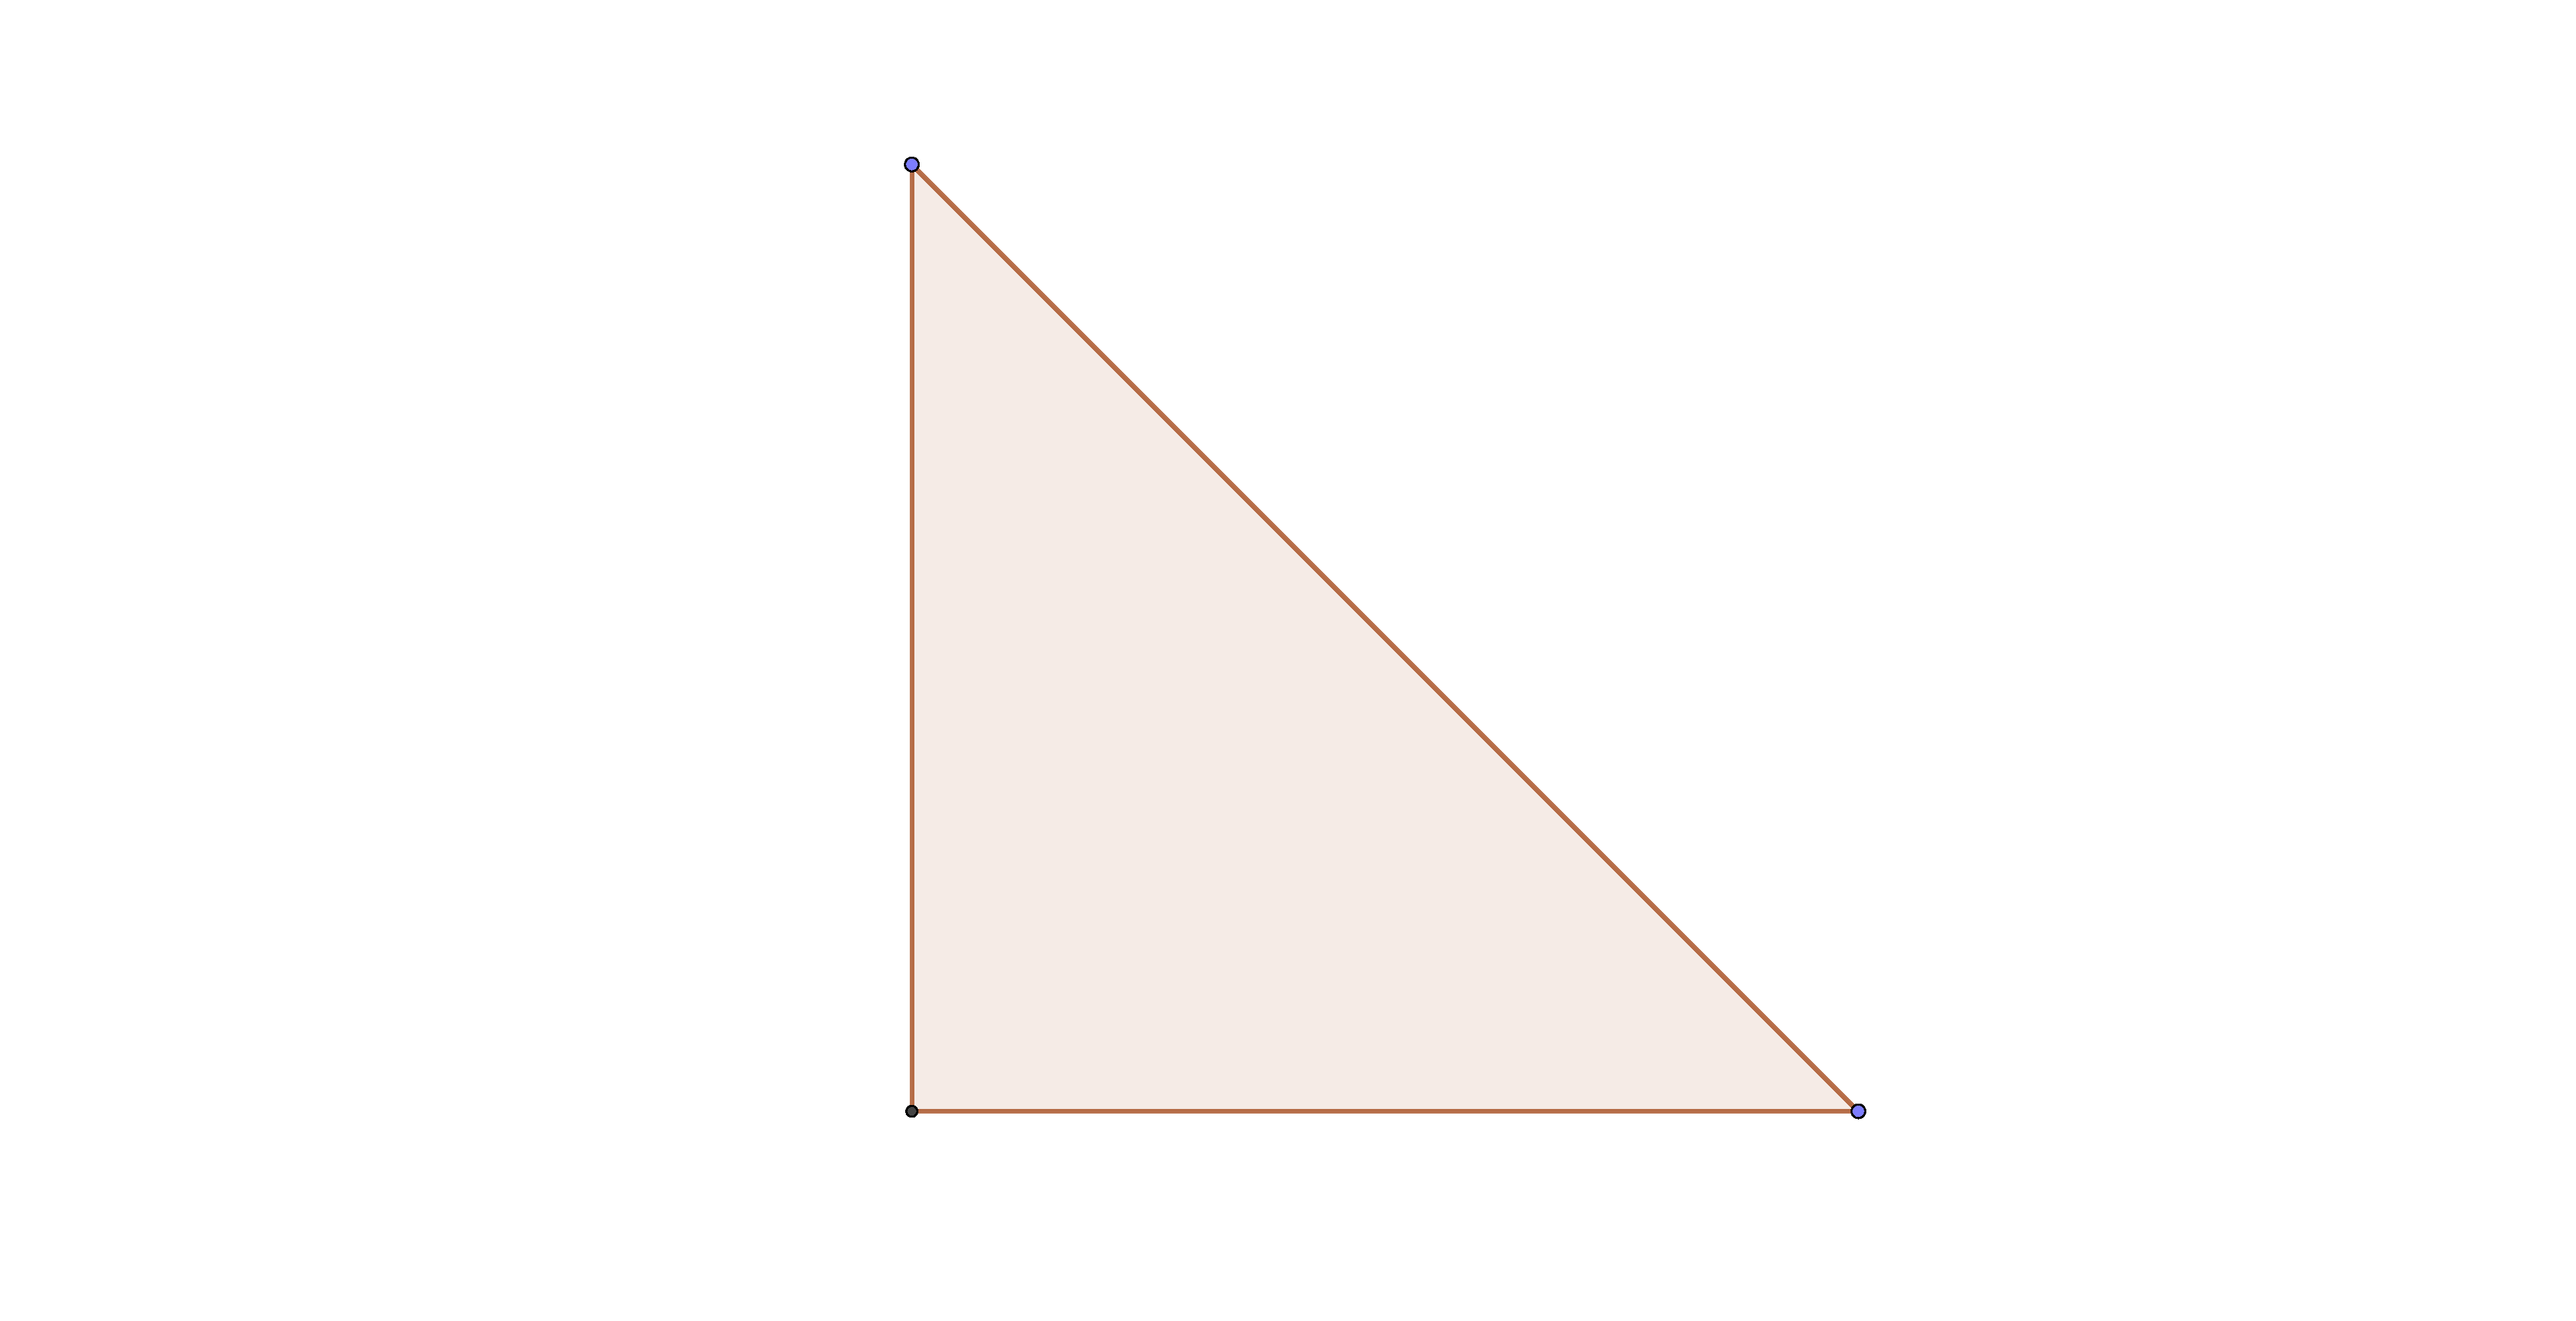
\includegraphics[width=.4\linewidth]{figures/cp2-polytope}
		\end{minipage}%
		\begin{minipage}{.3\textwidth}
			\centering
			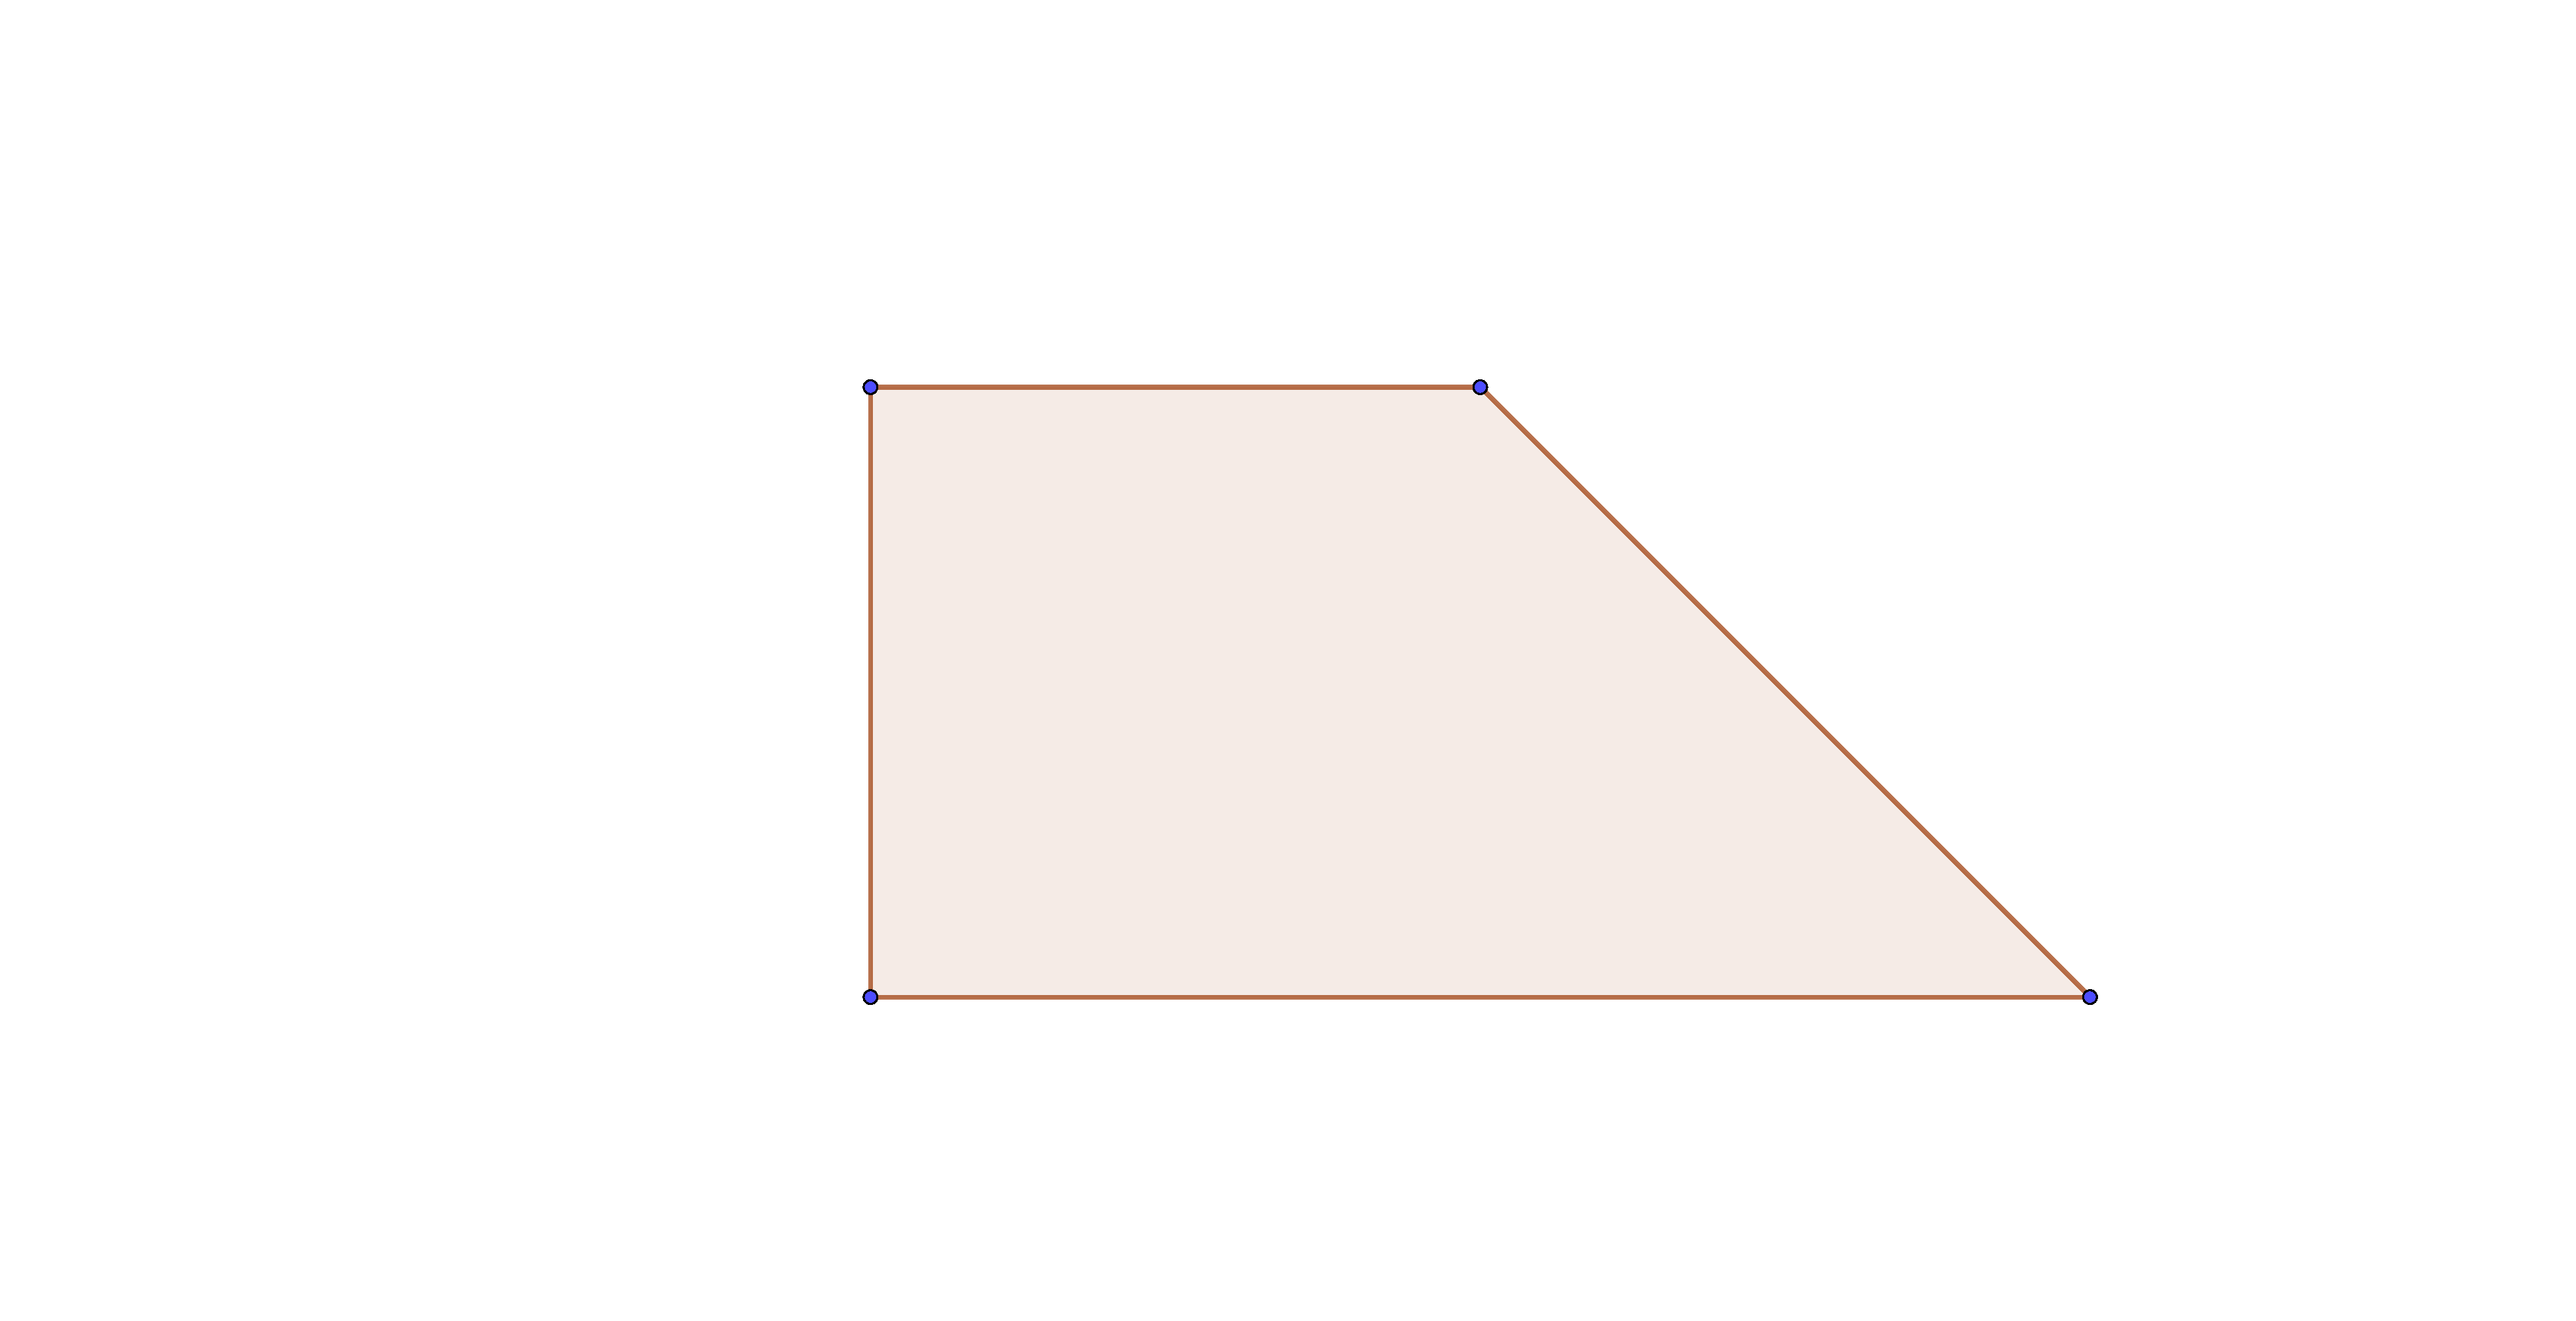
\includegraphics[height=.4\linewidth]{figures/blowup-polytope}
		\end{minipage}
		\hspace{-12pt}$\leftrightarrow$\ \reallywidetilde{\CC\PP^{2}}
	\end{figure}
\end{exs}

\end{frame}

%%%%%%%%%%%%%%%%%%%%%%%%%%%%%%%%%%%%%%%%%%%%%%%%
% Troisième diapo
%%%%%%%%%%%%%%%%%%%%%%%%%%%%%%%%%%%%%%%%%%%%%%%%
\begin{frame}
	\frametitle{Introduction \& Motivation}
	\framesubtitle{Delzant Construction}
	
	\begin{rmk}
		Given $(X^{2n}, \w, T^{n}, \mu)$, the Atiyah, Guillemin-Sternberg convexity theorem asserts that $\mu(X^{2n}) = \Delta \subset (\RR^{n})^{\ast}$ is a Delzant polytope.
	\end{rmk}
	
	\begin{thm}[Delzant]
		$$
		\frac{(X^{2n}, \w,T^{n},\mu)}{T^{n}\text{-equivariance}} \overset{1-1}{\longleftrightarrow} \frac{\text{Delzant polytopes}}{SL(n,\ZZ) \ltimes \RR^{n}}
		$$
	\end{thm}
	
	\begin{qstn}
		So for a given $\Delta \subset (\RR^{d})^{\ast}$, what is the respective $X_{\Delta}$?
	\end{qstn}


\end{frame}

%%%%%%%%%%%%%%%%%%%%%%%%%%%%%%%%%%%%%%%%%%%%%%%%
% Troisième diapo
%%%%%%%%%%%%%%%%%%%%%%%%%%%%%%%%%%%%%%%%%%%%%%%%
\begin{frame}
	\frametitle{Introduction \& Motivation}
	\framesubtitle{Delzant Construction}
	
	Let $u_{i}\in \RR^{d}$ $(i=1,\ldots,n)$ be the inward-pointing normals to to facets of $\Delta$, and define $\pi(e_{i}) = u_{i}$.
	
	\begin{equation*}
	\begin{tikzcd}[ampersand replacement=\&]
	0 \arrow[r] \& \mf{n}:= \ker \pi \arrow[r, "i",hook] \& \mathbb{R}^{n} \arrow[r, "\pi"] \& \mathbb{R}^{d} \arrow[r] \& 0
	\end{tikzcd}
	\end{equation*}
	Can dualise:
	\begin{equation*}
	\begin{tikzcd}[ampersand replacement=\&]
	0 \& \arrow[l] \mf{n}^{\ast} \& \arrow[l, "i^{\ast}",swap] (\mathbb{R}^{n})^{\ast} \& \arrow[l,"\pi^{\ast}",swap] (\RR^{d})^{\ast} \& \arrow[l] 0
	\end{tikzcd}
	\end{equation*}
	Or exponentiate:
	\begin{equation*}
	\begin{tikzcd}[ampersand replacement=\&]
	0 \arrow[r] \& N \arrow[r, "i",hook] \& T^{n} \arrow[r, "\pi"] \& T^{d} \arrow[r] \& 0
	\end{tikzcd}
	\end{equation*}
	
\end{frame}

%%%%%%%%%%%%%%%%%%%%%%%%%%%%%%%%%%%%%%%%%%%%%%%%
% Troisième diapo
%%%%%%%%%%%%%%%%%%%%%%%%%%%%%%%%%%%%%%%%%%%%%%%%
\begin{frame}
	\frametitle{Introduction \& Motivation}
	\framesubtitle{Delzant Construction}
	
	\begin{equation*}
	\begin{tikzcd}[ampersand replacement=\&]
	0 \arrow[r] \& N \arrow[r, "i",hook] \& T^{n} \arrow[r, "\pi"] \& T^{d} \arrow[r] \& 0
	\end{tikzcd}
	\end{equation*}
	
	$T^{n}$ acts diagonally on $\CC^{n}$, with moment map:
	$$
		J:\CC^{n} \rightarrow (\RR^{n})^{\ast},\qquad J(z) = \frac{1}{2}\sum_{i=1}^{n}(|z_{i}|^{2} - \lambda_{i})e_{i},\quad \lambda\in (\RR^{n})^{\ast}.
	$$
	$N$ also acts on $\CC^{n}$ via inclusion, with moment map $i^{\ast}\circ J: \CC^{n} \rightarrow \mf{n}^{\ast}$.
	
	
	\begin{fact}
		$X_{\Delta} := (i^{\ast}\circ J)^{-1}(0) / N$ is a toric symplectic manifold for the residual $T^{d}$-action, with Delzant polytope $\Delta$, where $$\Delta = \cap_{i=1}^{n} \{y \in \RR^{d} \st \langle y, u_{i} \rangle \geq \lambda_{i} \text{ for all } i  \}.$$
	\end{fact}
	
\end{frame}


%%%%%%%%%%%%%%%%%%%%%%%%%%%%%%%%%%%%%%%%%%%%%%%%
% Troisième diapo
%%%%%%%%%%%%%%%%%%%%%%%%%%%%%%%%%%%%%%%%%%%%%%%%
\begin{frame}
\frametitle{Introduction \& Motivation}
\framesubtitle{Geometric Quantisation}

\begin{qstn}
	For a (pre-quantum) line bundle $\mc{L}$ over $(X,\w)$, can one find a canonical Hilbert space of (holomorphic) ``wave-functions'' $\mc{Q}(X)$ with 
	$$
		\mc{Q}(X) = H^{0}(X,\mc{L})?
	$$
\end{qstn}

\begin{conj}[``Quantisation Commutes with Reduction'']
	If $X_{0} = \mu^{-1}(0)/G$, then:
	$$
		\mc{Q}(X)^{G} = \mc{Q}(X_{0})
	$$
	Further, if $X_{\alpha} = \mu^{-1}(\alpha)/G$:
	$$
		\dim \mc{Q}(X_{\alpha}) = \mult(\alpha)
	$$
\end{conj}

\end{frame}


%%%%%%%%%%%%%%%%%%%%%%%%%%%%%%%%%%%%%%%%%%%%%%%%
% Troisième diapo
%%%%%%%%%%%%%%%%%%%%%%%%%%%%%%%%%%%%%%%%%%%%%%%%
\begin{frame}
	\frametitle{Introduction \& Motivation}
	\framesubtitle{Lattice Point Counting}
	
	\begin{thm}
	For toric symplectic manifolds:
	$
		\dim \mc{Q}(X) = \#(\Delta \cap \ZZ^{n})
	$
	\end{thm}

	\begin{ex}
		$X = \CC^{3}$ and $\CC\PP^{2} = X_{k} = \mu^{-1}(k)/N$. For $s:\CC^{3} \rightarrow \CC$ holomorphic, locally $s(z) = z_{0}^{j_{0}}z_{1}^{j_{1}}z_{2}^{j_{2}}$. For $N$-equivariance:
		\vspace{-10pt}
		$$
			s(n\cdot z) = n^{j_{0} + j_{1} + j_{2}}s(z) \overset{?}{=} n\cdot s(z) = n^{k}s(z).
		$$
		True for $H^{0}(\CC\PP^{2},\mc{O}(k))$, and solution set:
		$$
			\{(j_{0}, j_{1}, j_{2}) \st \sum j_{i} = k  \} \overset{1-1}{\leftrightarrow} \{(j_{0}, j_{2})\st j_{0} + j_{1} \leq k  \} \equiv (\Delta \cap \ZZ^{2}).
		$$
	\end{ex}

\end{frame}

%%%%%%%%%%%%%%%%%%%%%%%%%%%%%%%%%%%%%%%%%%%%%%%%
% Troisième diapo
%%%%%%%%%%%%%%%%%%%%%%%%%%%%%%%%%%%%%%%%%%%%%%%%
\begin{frame}
		\frametitle{Introduction \& Motivation}
		\framesubtitle{The Verlinde Formula}
		
	\begin{rmk}
		Case for $X = \CC^{4}$ and $X_{k} = \mu^{-1}(k)/N \cong \CC\PP^{3}$ very similar, with Delzant polytope $k\Delta \subset \RR^{3}$ ($\Delta$ the standard $3$-simplex).
		$$
		\#(k\Delta \cap \ZZ^{3}) = \frac{(k+1)(k+2)(k+3)}{3!} = \frac{k^{3}}{6} + k^{2} + \frac{11}{6}k + 1.
		$$
	\end{rmk}

	\begin{fact}
		Let $M = \mc{M}_{\text{flat}}(\Sigma_{2};SU(2))$, and $\mc{L}$ be the determinant line bundle. Then:
		$$
			\dim H^{0}(M,\mc{L}^{\otimes k}) = \#(k\Delta \cap \ZZ^{3}).
		$$
		In fact, $M \cong \CC\PP^{3}$, and the above equation is known as the \emph{Verlinde formula} for $M$.
	\end{fact}	

\end{frame}

%%%%%%%%%%%%%%%%%%%%%%%%%%%%%%%%%%%%%%%%%%%%%%%%
% Troisième diapo
%%%%%%%%%%%%%%%%%%%%%%%%%%%%%%%%%%%%%%%%%%%%%%%%
\begin{frame}
	\frametitle{Introduction \& Motivation}
	\framesubtitle{Higgs Bundle Moduli}
	
	\begin{qstn}
		What about the moduli space for Higgs bundle $\mc{M}_{\text{Higgs}}(\Sigma_{g};G)$, which is \emph{non-compact}?
	\end{qstn}

	It has $T^{\ast}\mc{M}_{\text{flat}}(\Sigma_{g};G) \subset \mc{M}_{\text{Higgs}}(\Sigma_{g};G)$ as an open and dense subset.
	As $\mc{M}_{\text{Higgs}}$ is non-compact, $\dim \mc{Q}(\mc{M}_{H}) = \infty$.
	However $\mc{M}_{H}$ admits a $\CC^{\ast}$-action by scaling the Higgs fields, and $S^{1}\subset \CC^{\ast}$ has compact fixed point loci $\implies \CC^{\ast}$-weight decomposition:
	$$
	\mc{Q}(\mc{M}_{H}) = \bigoplus_{n\geq 0}\mc{Q}(\mc{M}_{H})_{n}.
	$$
	
\end{frame}

%%%%%%%%%%%%%%%%%%%%%%%%%%%%%%%%%%%%%%%%%%%%%%%%
% Troisième diapo
%%%%%%%%%%%%%%%%%%%%%%%%%%%%%%%%%%%%%%%%%%%%%%%%
\begin{frame}
	\frametitle{Introduction \& Motivation}
	\framesubtitle{The Equivariant Verlinde Formula}

	\begin{prop}
		The \emph{equivariant Verlinde formula} is a recipe for calculating the $n$\textsuperscript{th} graded part for $\dim \mc{Q}(\mc{M}_{\text{Higgs}})$, \ie 
		$$
			\dim_{t} H^{0}(\mc{M}_{H},\mc{L}^{k}) = \sum_{n=0}^{\infty}\dim H_{n}^{0}(\mc{M}_{H},\mc{L}^{k})t^{n}.
		$$
		\end{prop}	
	In particular, the degree-0 (weight-0) part corresponds to the classical Verlinde formula.
	
	\begin{rmk}
		There is also an equivariant Verlinde formula for \emph{parabolic Higgs bundles}.
	\end{rmk}
\end{frame}
	
	% La 2e partie: Le point de vue de la relativité restreinte
	% Titre de la premiere partie
\section[]{My Progress}

%%%%%%%%%%%%%%%%%%%%%%%%%%%%%%%%%%%%%%%%%%%%%%%%
% Première diapo
%%%%%%%%%%%%%%%%%%%%%%%%%%%%%%%%%%%%%%%%%%%%%%%%
\begin{frame}
\frametitle{Toric Hyperk{\"a}hler Manifolds \& Compactification}
\framesubtitle{Hyperk{\"a}hler Analogues}

Complexification analogy for toric symplectic manifolds are \emph{hypertoric} manifolds: consider $M = T^{\ast}\CC^{n}$ with induced linear $G$-action from $\CC^{n}$, and moment map $\mu:\CC^{n} \rightarrow \mf{g}^{\ast}$.

Action is hyperhamiltonian with \HK moment map $\mu_{HK} := \mu_{\RR} \oplus \mu_{\CC}:T^{\ast}\CC^{n} \rightarrow \mf{g}^{\ast} \oplus \mf{g}_{\CC}^{\ast}$, where:
$$
	\mu_{\RR}(z,w) = \mu(z) - \mu(w),\qquad \mu_{\CC}(z,w)(v) =w(\hat{v}_{z}),
$$
with $w\in T_{z}^{\ast}\CC^{n}$, $v \in \mf{g}_{\CC}$, and $\hat{v}_{z} \in T_{z}\CC^{n}$ induced.
\begin{defn}
	For $\alpha \in Z(\mf{g}^{\ast})$:
	$$
		M := (\mu_{\RR}^{-1}(\alpha)\cap \mu_{\CC}^{-1}(0))/G
	$$
	is the \emph{hyperk{\"a}hler analogue} to the K{\"a}hler $X = \mu^{-1}(\alpha)/G$.
\end{defn}

\end{frame}

%%%%%%%%%%%%%%%%%%%%%%%%%%%%%%%%%%%%%%%%%%%%%%%%
% Première diapo
%%%%%%%%%%%%%%%%%%%%%%%%%%%%%%%%%%%%%%%%%%%%%%%%
\begin{frame}
	\frametitle{Toric Hyperk{\"a}hler Manifolds \& Compactification}
	\framesubtitle{Toric Hyperk{\"a}hler Manifolds}
	
	Let $X = \mu^{-1}(\alpha)/N$ be a symplectic toric manifold with a residual $T^{d} = T^{n}/N$ action from the Delzant construction.
	\begin{defn}
		A \emph{toric hyperk{\"a}hler manifold} $M$ is the hyperk{\"a}hler analogue to the K{\"a}hler quotient $X$.
	\end{defn}
	Explicitly:
	$$
		M = (\mu_{\RR}^{-1}(\alpha) \cap \mu_{\CC}^{-1}(0))/N,
	$$
	and, if $i^{\ast}(r_{1},\ldots, r_{n}) = \alpha$ and $(\partial_{i})_{i=1}^{n}$ is a basis for $(\RR^{d})^{\ast} = \ker i^{\ast}$, we get residual moment maps:
	$$
		\phi_{\RR}[z,w] = \frac{1}{2}\sum_{i=1}^{n}(|z_{i}|^{2} - |w_{i}|^{2} - r_{i})\partial_{i},\qquad \phi_{\CC}[z,w] = \sum_{i=1}^{n}(z_{i}w_{i})\partial_{i}.
	$$
\end{frame}

%%%%%%%%%%%%%%%%%%%%%%%%%%%%%%%%%%%%%%%%%%%%%%%%
% Première diapo
%%%%%%%%%%%%%%%%%%%%%%%%%%%%%%%%%%%%%%%%%%%%%%%%
\begin{frame}
	\frametitle{Toric Hyperk{\"a}hler Manifolds \& Compactification}
	\framesubtitle{The Extended Core}

\begin{defn}
	The set
	$$
		\mc{E} := \phi_{\CC}^{-1}(0) = \{[z,w] \in M \st z_{i}w_{i} = 0 \}
	$$
	is called the \emph{extended core} of $M$.
\end{defn}

For each $A \subseteq \{1,\ldots, n\}$, $\mc{E}$ breaks up into components:
$$
\mc{E}_{A} = \{[z,w] \in M \st w_{i} = 0 \text{ if } i \in A, \text{ and } z_{i} = 0 \not\in A   \},
$$ 
with image
$$
\Delta_{A} := \phi_{\RR}(\mc{E}_{A}) = \bigcap_{i \in A}F_{i} \cap \bigcap_{i\not\in A} G_{i}, 
$$
for
$$
	F_{i} = \{y \in (\RR^{d})^{\ast}\st \langle y, u_{i}\rangle + r_{i} \geq 0 \},\quad G_{i} = \{y \in (\RR^{d})^{\ast}\st \langle y,u_{i}\rangle + r_{i} \leq 0 \}.
$$

\end{frame}

%%%%%%%%%%%%%%%%%%%%%%%%%%%%%%%%%%%%%%%%%%%%%%%%
% Première diapo
%%%%%%%%%%%%%%%%%%%%%%%%%%%%%%%%%%%%%%%%%%%%%%%%
\begin{frame}
	\frametitle{Toric Hyperk{\"a}hler Manifolds \& Compactification}
	\framesubtitle{Example, $T^{\ast}\CC\PP^{2}$}

	\begin{figure}
		\centering
		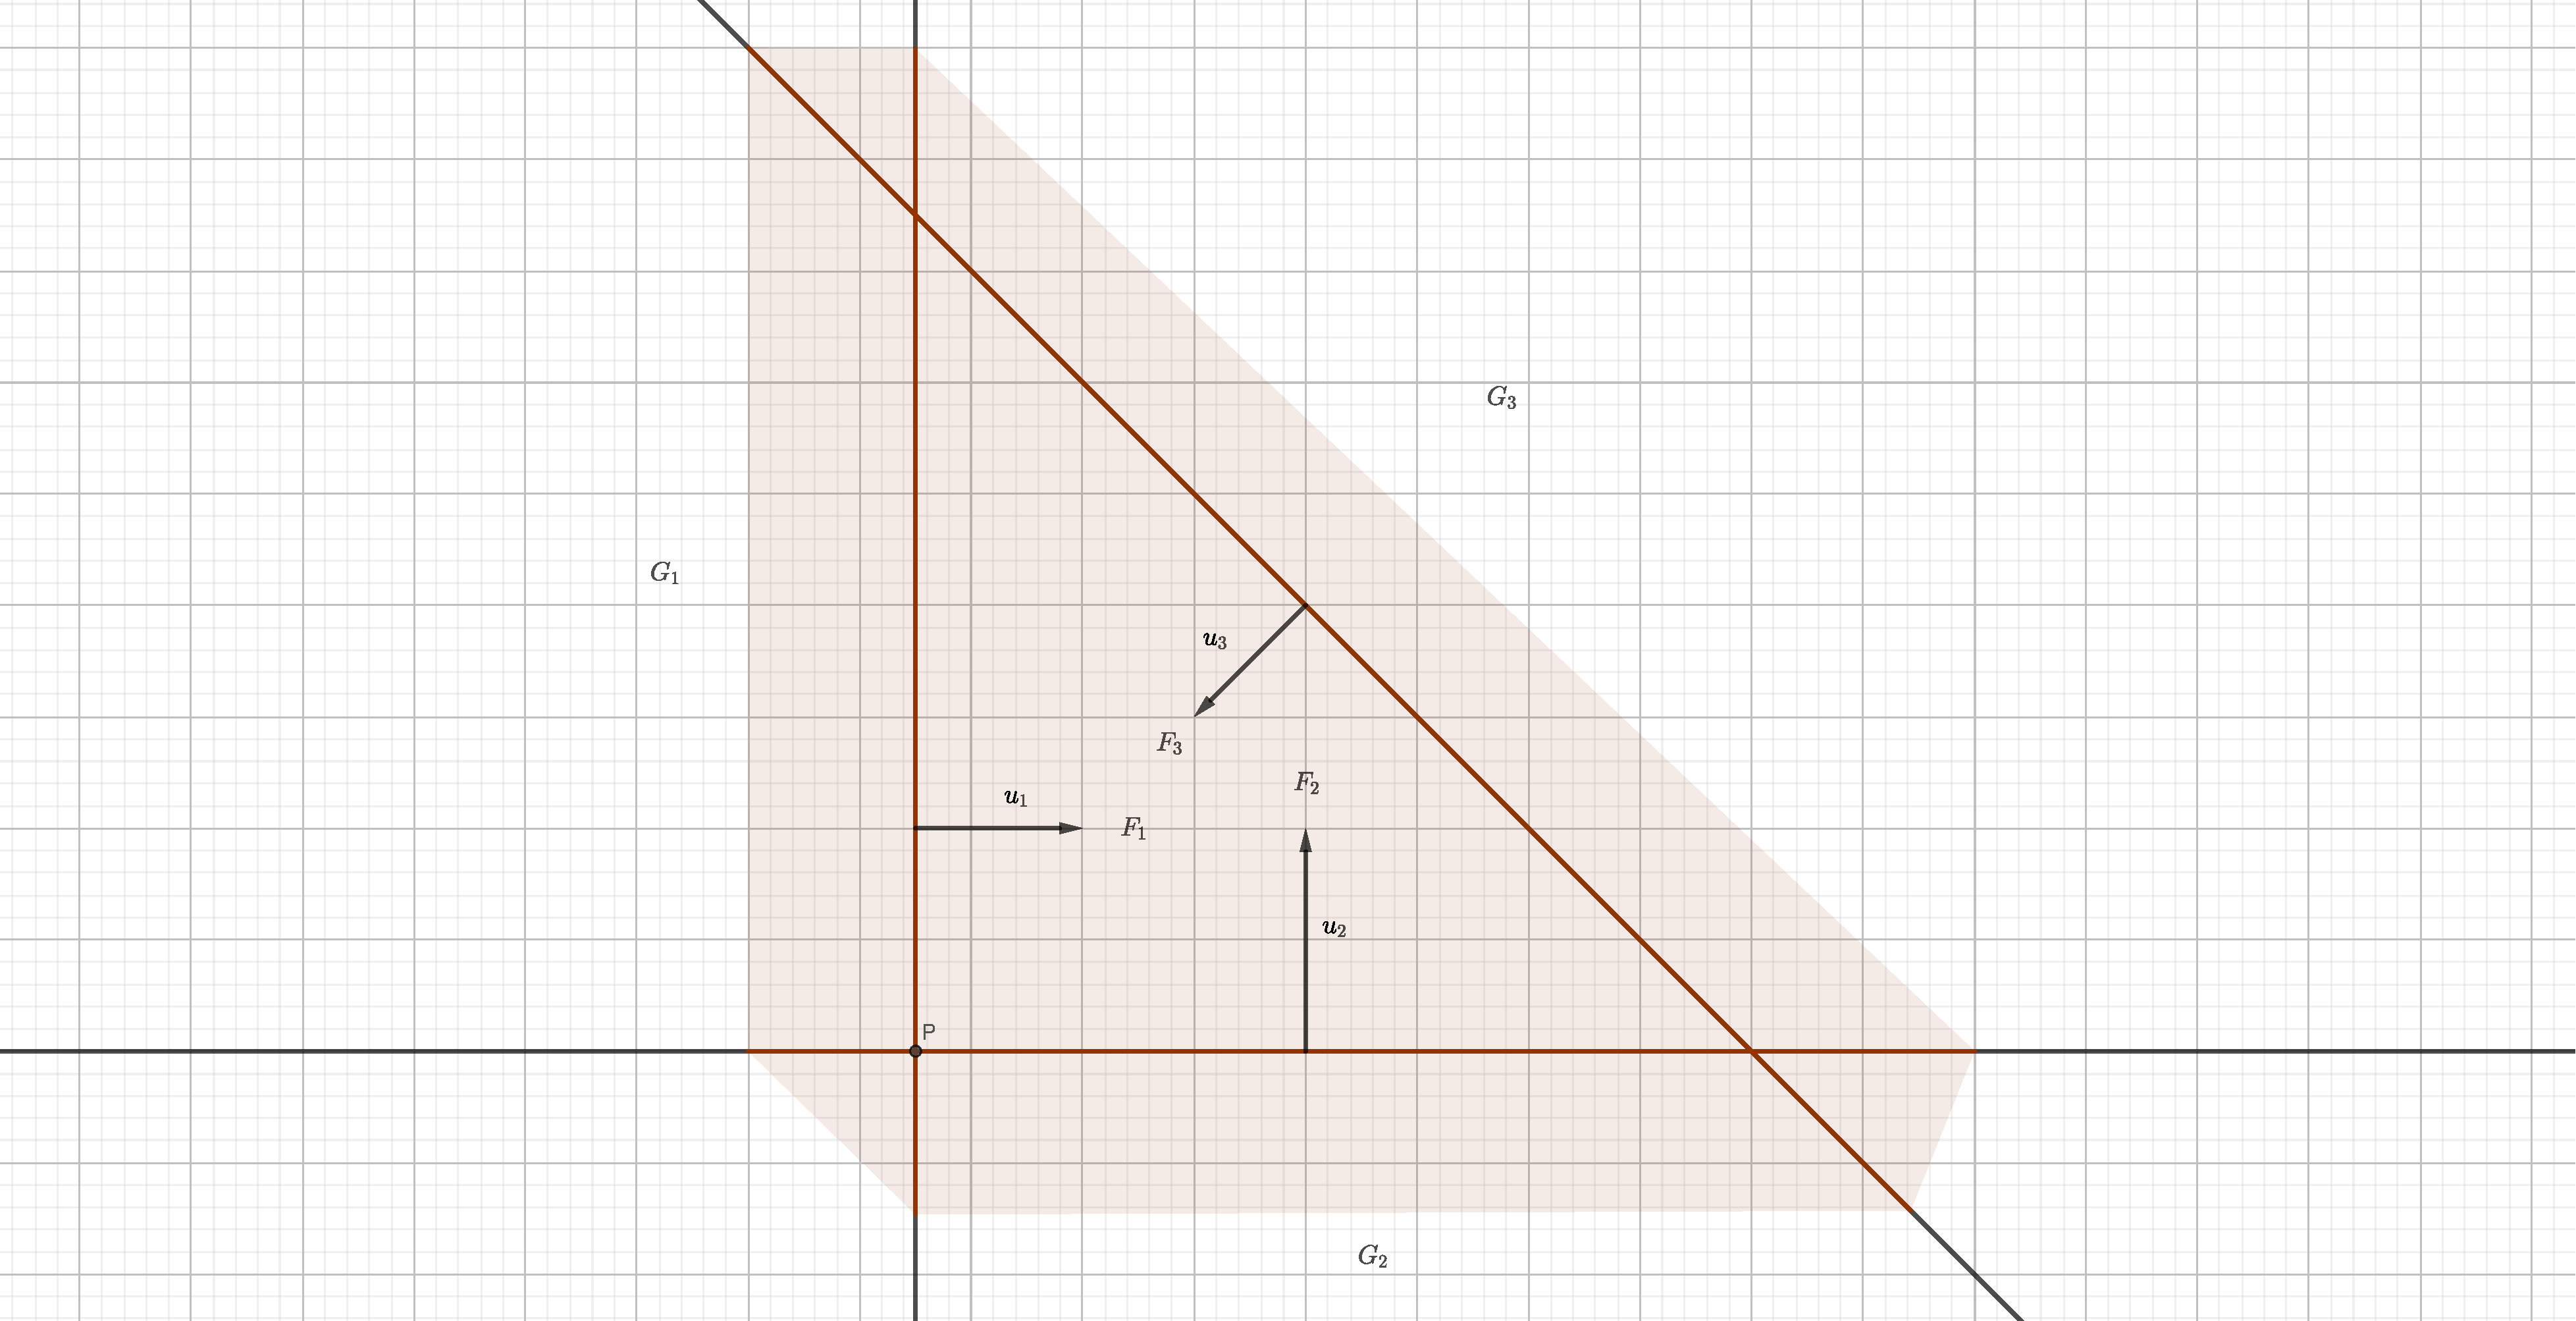
\includegraphics[width=1.2\linewidth]{figures/cp2-components}
	\end{figure}

\end{frame}

%%%%%%%%%%%%%%%%%%%%%%%%%%%%%%%%%%%%%%%%%%%%%%%%
% Première diapo
%%%%%%%%%%%%%%%%%%%%%%%%%%%%%%%%%%%%%%%%%%%%%%%%
\begin{frame}
	\frametitle{Toric Hyperk{\"a}hler Manifolds \& Compactification}
	\framesubtitle{Residual Circle Action}
	$$
		S^{1}\text{-action:}\qquad\hbar\cdot [z,w] = [z,\hbar w],\qquad \hbar \in S^{1}.
	$$
	Descends to $\mc{E}$ and, on each $\mc{E}_{A}$, acts as a subgroup of $T^{n}$. On $\mc{E}_{A}$:
	$$
		[z,\hbar w] = [\hbar^{-1}z_{1}, \ldots, \hbar^{-1}z_{n}; w] = [\hbar_{1}z_{1},\ldots, \hbar_{n}z_{n}; w],
	$$
	with
	$$
	\hbar_{i} :=
		\begin{cases}
		\hbar^{-1},\quad &\text{if } i \in A,\\
		1,\quad &\text{if } i \not\in A.
		\end{cases}
	$$
	For $j_{A}:\restr{S^{1}}{\mc{E}_{A}} \hookrightarrow T^{n}$, its moment map is
	$$
		\Phi_{A}[z,w] = -\bigg\langle \mu_{\RR}[z,w], \sum_{i\in A} u_{i} \bigg\rangle.
	$$
\end{frame}

%%%%%%%%%%%%%%%%%%%%%%%%%%%%%%%%%%%%%%%%%%%%%%%%
% Première diapo
%%%%%%%%%%%%%%%%%%%%%%%%%%%%%%%%%%%%%%%%%%%%%%%%
\begin{frame}
	\frametitle{Toric Hyperk{\"a}hler Manifolds \& Compactification}
	\framesubtitle{Compactification via Symplectic Cutting}
	
	Globally $\Phi[z,w] = \tfrac{1}{2}\|w\|^{2}$ is proper; can ``compactify'' $M$: let $S^{1}$ act on $M \times \CC$ diagonally. Moment map:
	$$
		\mu_{\text{cut}}:M \times \CC \rightarrow \RR,\qquad ([z,w],\xi) \mapsto \Phi[z,w] + \tfrac{1}{2}|\xi|^{2}.
	$$
	Resulting in:
	$$
	M_{\epsilon} := \mu_{\text{cut}}^{-1}(\epsilon)/S^{1} \cong \{m\in M \st \Phi(m) < \epsilon \} \sqcup \Phi^{-1}(\epsilon)/S^{1}
	$$
	On each component $\mc{E}_{A}^{(\epsilon)} := \mc{E}_{A} \cap M_{\epsilon}$, we find that:
	$$
		\phi_{\RR}(\mc{E}_{A}^{(\epsilon)}) = \Delta_{A} \cap \{ v \in (\RR^{d})^{\ast} \st \langle v, {\scriptstyle\sum}_{i\in A} u_{i} \rangle \leq \e   \}
	$$
\end{frame}

%%%%%%%%%%%%%%%%%%%%%%%%%%%%%%%%%%%%%%%%%%%%%%%%
% Première diapo
%%%%%%%%%%%%%%%%%%%%%%%%%%%%%%%%%%%%%%%%%%%%%%%%
\begin{frame}
	\frametitle{Toric Hyperk{\"a}hler Manifolds \& Compactification}
	\framesubtitle{Example for $T^{\ast}\CC\PP^{2}$}
	
	\begin{figure}
		\centering
		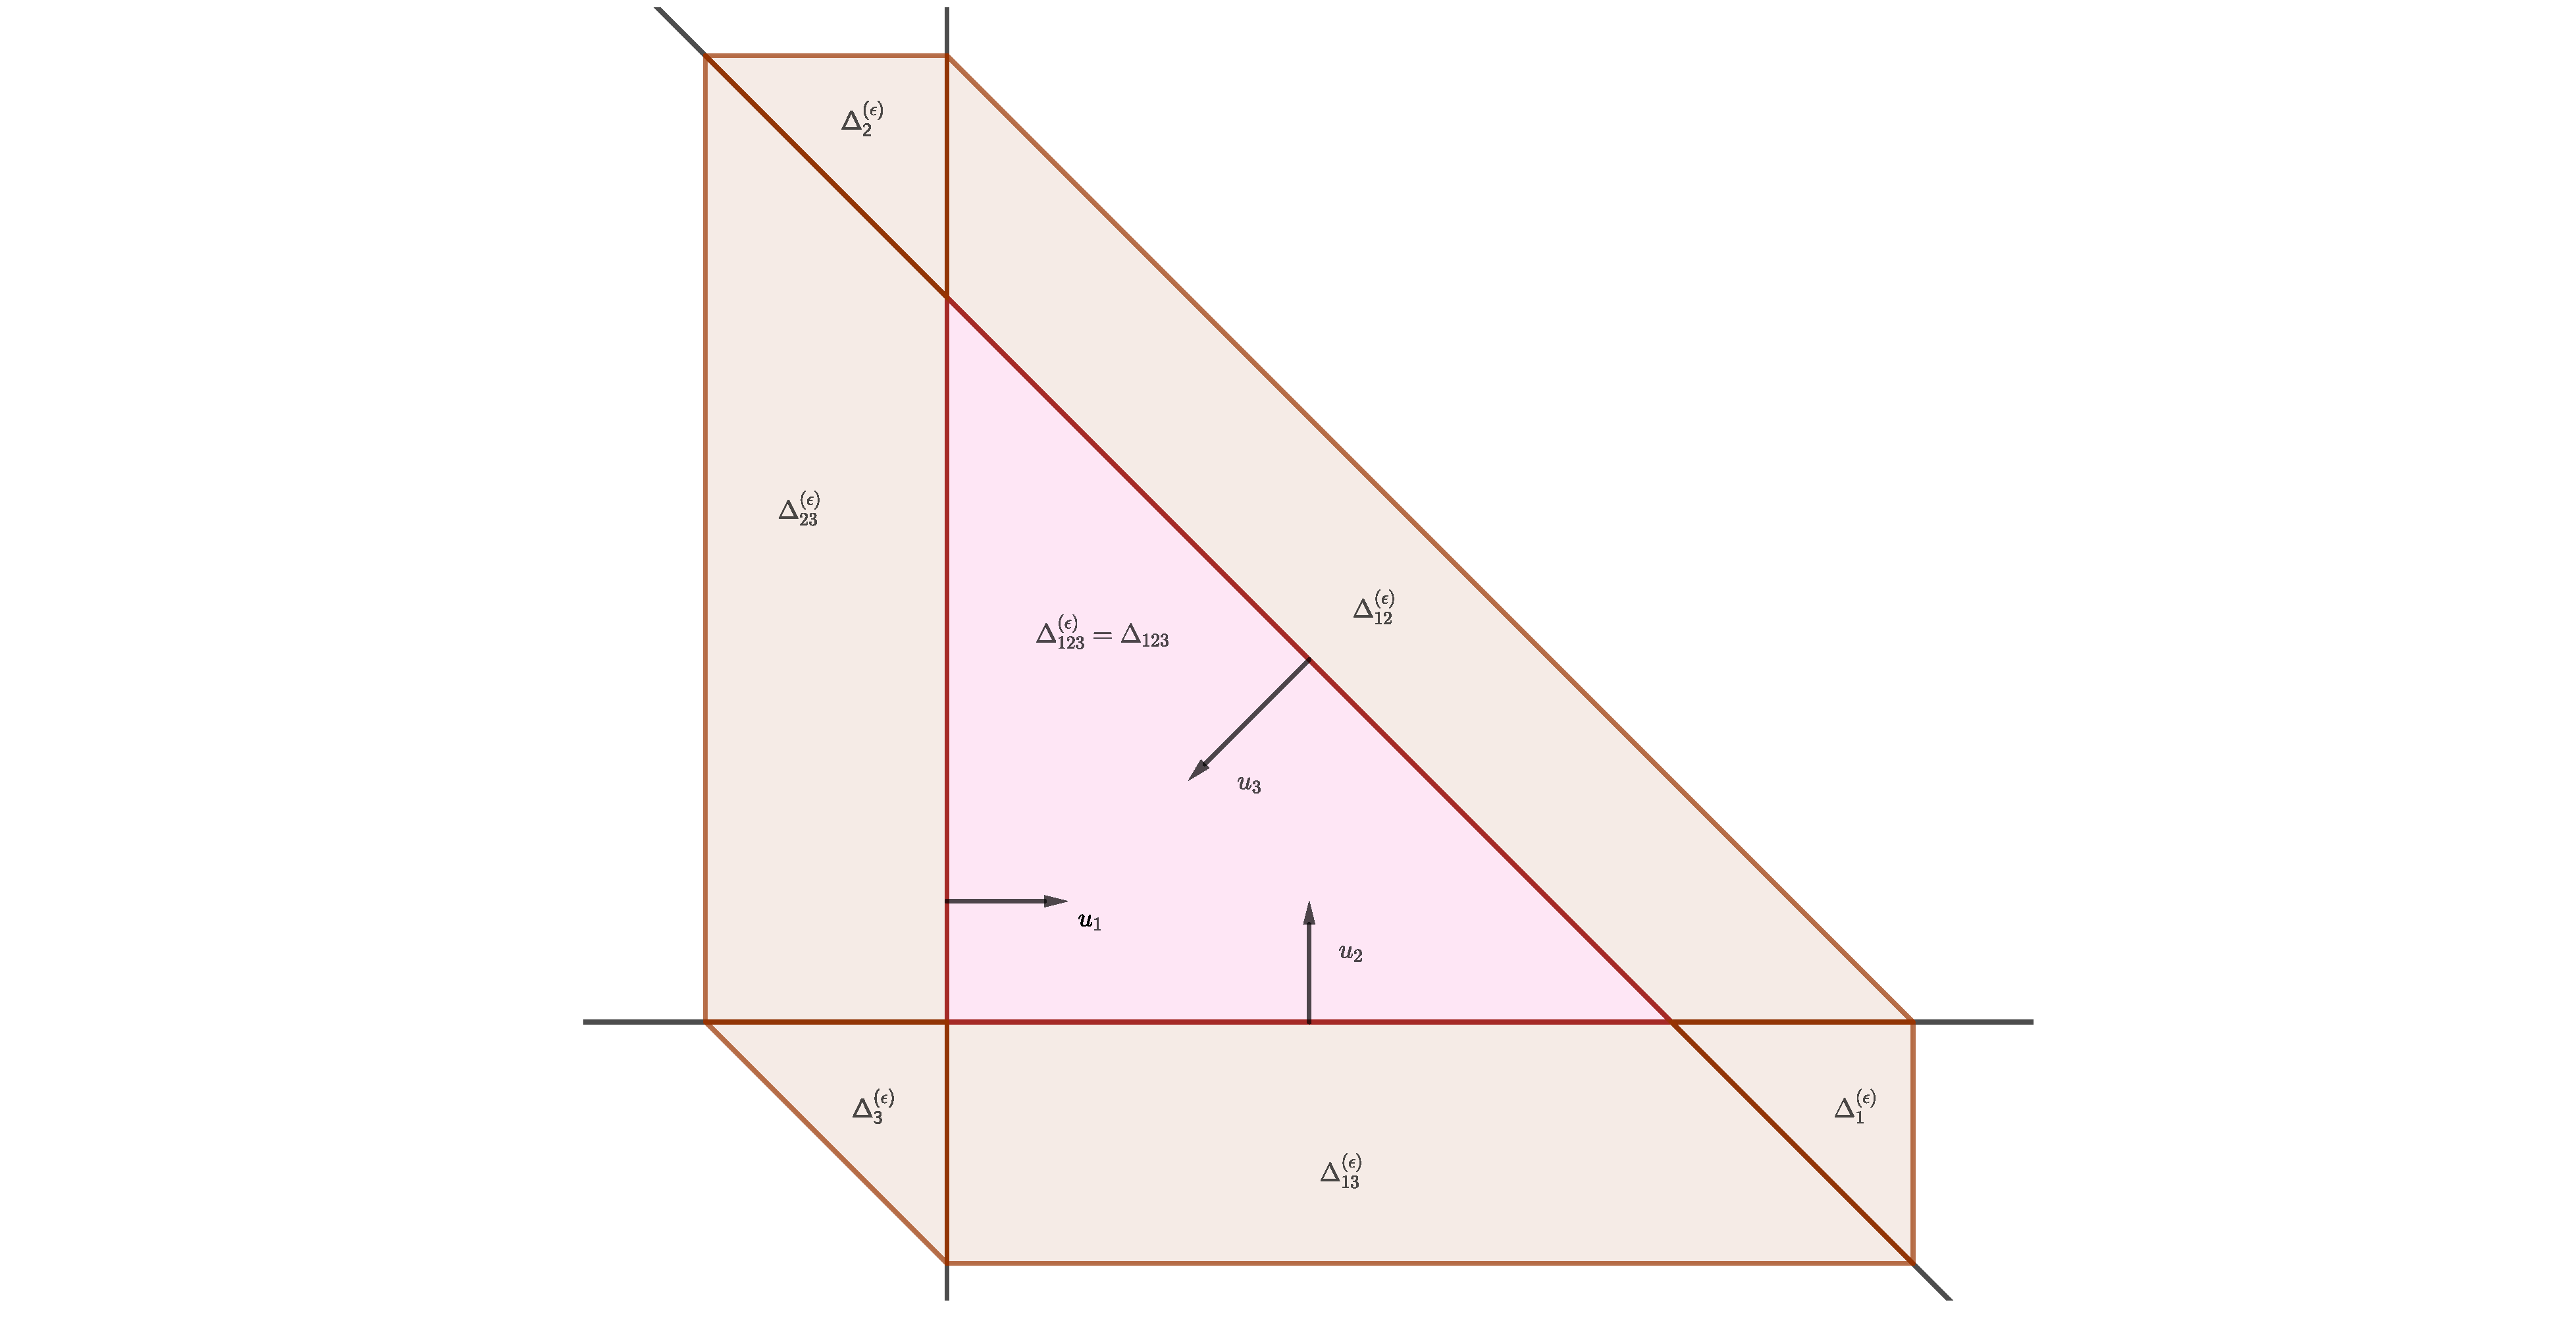
\includegraphics[width=0.7\linewidth]{figures/Symplectic_Cut_Cotangent_CP2}
	\end{figure}

\end{frame}

%%%%%%%%%%%%%%%%%%%%%%%%%%%%%%%%%%%%%%%%%%%%%%%%
% Première diapo
%%%%%%%%%%%%%%%%%%%%%%%%%%%%%%%%%%%%%%%%%%%%%%%%
\begin{frame}
	\frametitle{Toric Hyperk{\"a}hler Manifolds \& Compactification}
	\framesubtitle{Example for $T^{\ast}\CC\PP^{3}$}
	
	\begin{figure}
		\centering
		\begin{subfigure}{.5\textwidth}
			\centering
			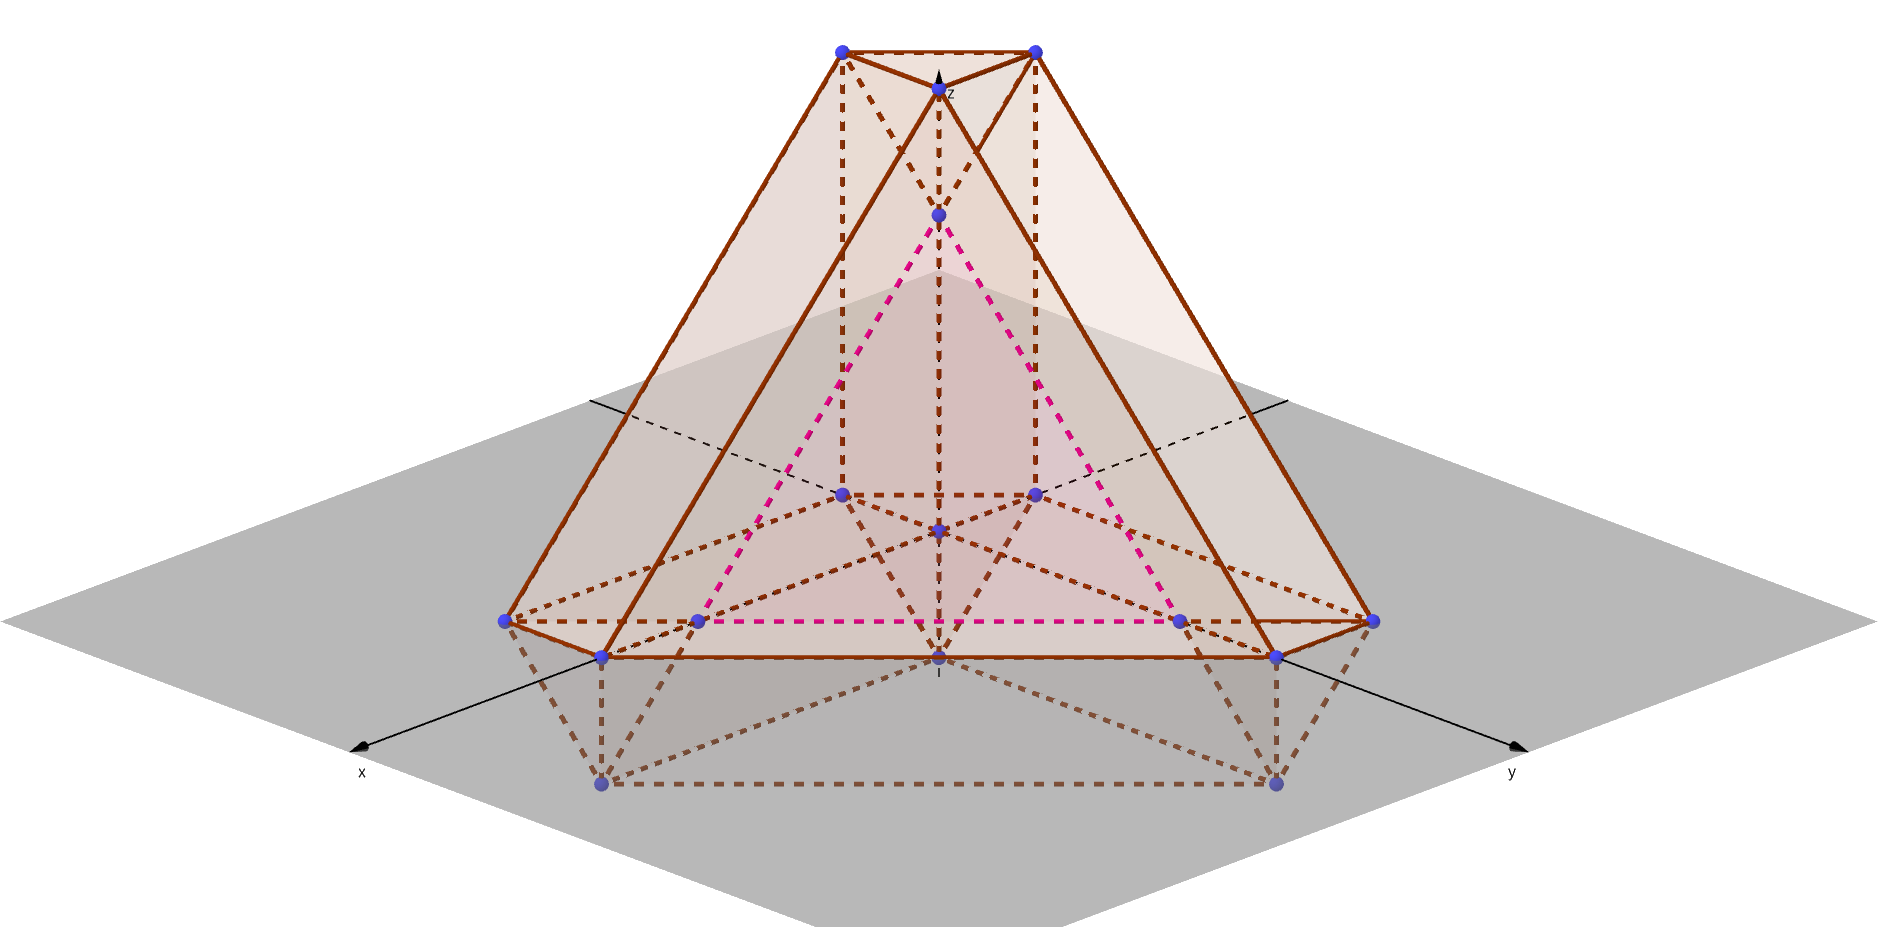
\includegraphics[width=1.2\linewidth]{figures/Symplectic_Cut_Cotangent_CP3.png}
		\end{subfigure}%
		\begin{subfigure}{.5\textwidth}
			\centering
			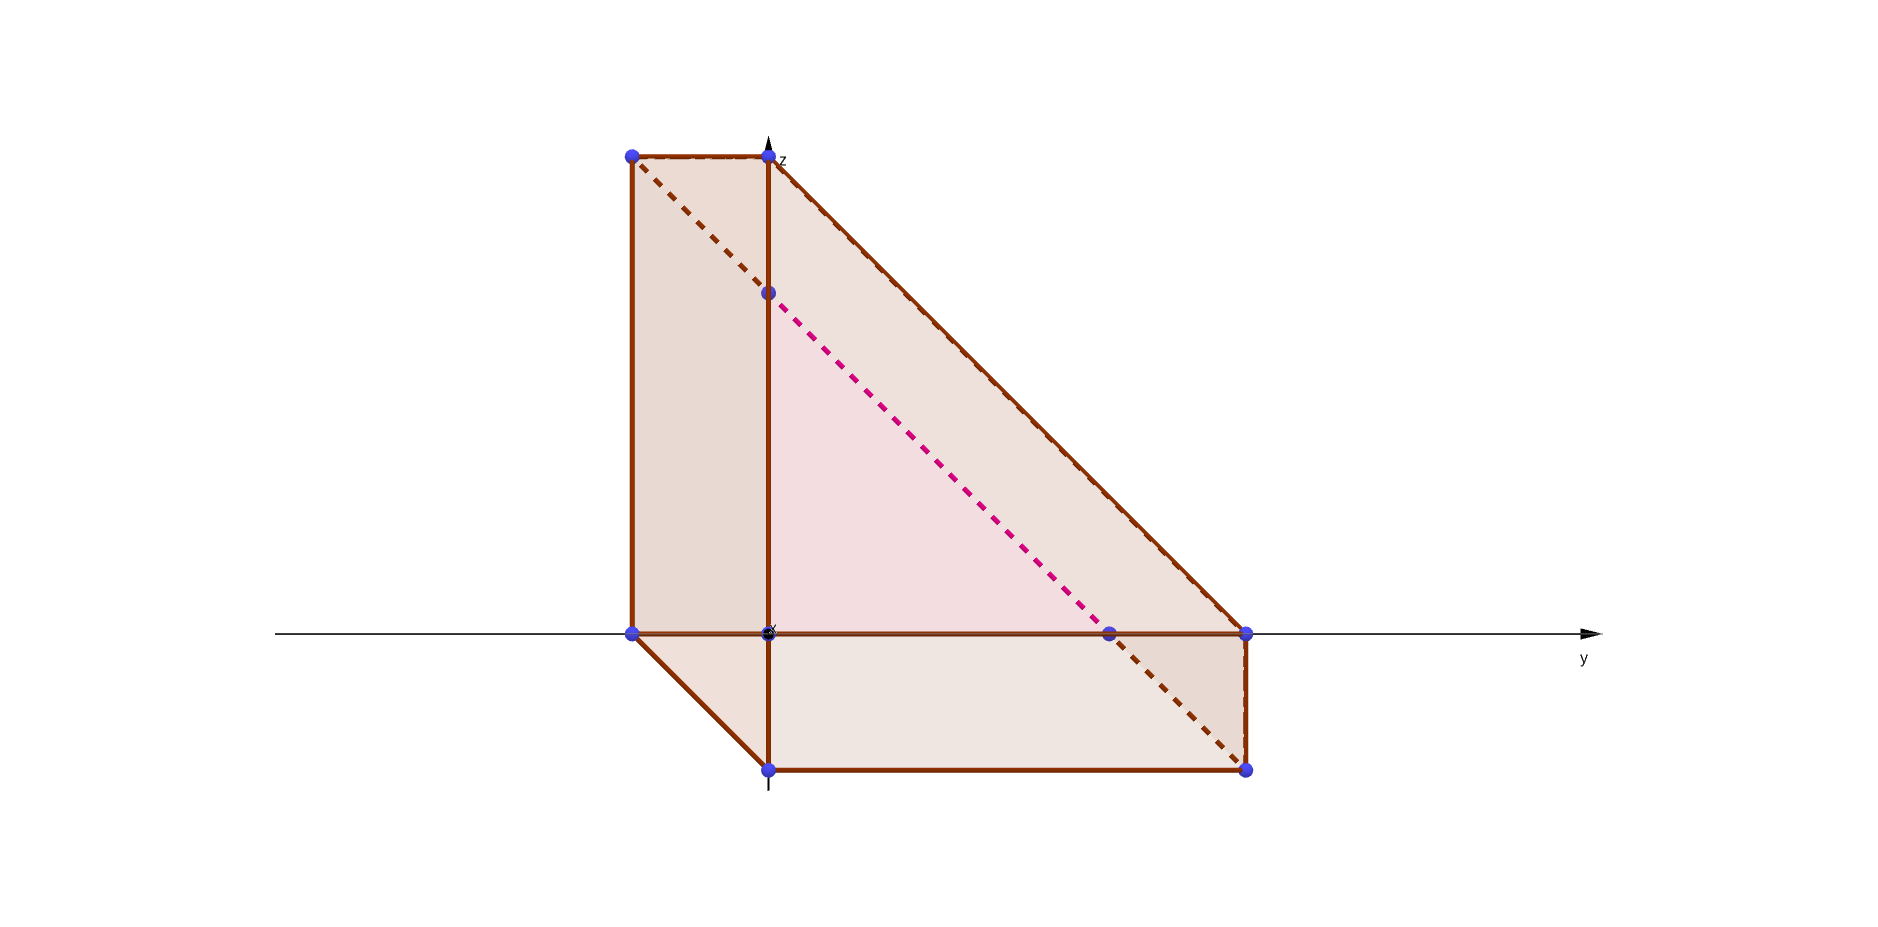
\includegraphics[width=1.2\linewidth]{figures/Symplectic_Cut_Cotangent_CP3-side.png}
		\end{subfigure}
	\end{figure}
	
	
\end{frame}



	
	% La 3e partie: Le point de vue de la relativité générale
	% Titre de la premiere partie
\section[]{Outlook}

%%%%%%%%%%%%%%%%%%%%%%%%%%%%%%%%%%%%%%%%%%%%%%%%
% Première diapo
%%%%%%%%%%%%%%%%%%%%%%%%%%%%%%%%%%%%%%%%%%%%%%%%
\begin{frame}
	\frametitle{Outlook}
	\framesubtitle{Toy Model Example}
	\begin{equation*}
		\begin{split}
					&\text{Recall:}\qquad G=SU(2),\quad G_{\CC} = SL(2,\CC),\quad g=2, \\
					&\text{and}\qquad\mc{M}_{\text{Higgs}}(\Sigma_{2};SU(2)) \cong T^{\ast}\CC\PP^{3}.
		\end{split}
	\end{equation*}

	\begin{ex}
		For ``large enough $k$'':
		\begin{equation*}
		\begin{split}
			\dim \mc{Q}(\mc{M}_{\text{Higgs}}(\Sigma_{2};G,k)) &= \frac{1}{6}k^{3} + k^{2} + \frac{11}{6}k + 1 \\
			&+ \bigg( \frac{1}{2}k^{3} + 3k^{2} - \frac{1}{2}k - 3  \bigg)t \\
			&+ (k^{3} + 8k^{2} -3k + 6) t^{2} + \ldots
		\end{split}
		\end{equation*}
	\end{ex}
	
	The degree-0 part is our classical Verlinde formula for $\CC\PP^{3}$.
	
\end{frame}

%%%%%%%%%%%%%%%%%%%%%%%%%%%%%%%%%%%%%%%%%%%%%%%%
% Première diapo
%%%%%%%%%%%%%%%%%%%%%%%%%%%%%%%%%%%%%%%%%%%%%%%%
\begin{frame}
	\frametitle{Outlook}
	\framesubtitle{A \emph{Hypertoric - Higgs Bundle} Lexicon}
	
	There are many striking analogies between hypertoric varieties and Higgs moduli spaces:
	\begin{table}[]
		\begin{tabular}{|l|l|}
			\hline
			Hypertoric Varieties, $M$ & Higgs Bundle Moduli, $\mathcal{M}_{\text{Higgs}}$   \\ \hline
			$\CC^{\ast}$-action  & Hitchin $\CC^{\ast}$-action                          \\ \hline
			$\Phi[z,w] = \tfrac{1}{2}\|w\|^{2}$, perfect Morse & $\mu(\mc{E},\phi) = \|\phi\|_{L^{2}}^{2}$, perfect Morse 							\\ \hline
			$T^{\ast}X \subset M$ open, dense & $T^{\ast}\mc{M}_{\text{\text{flat}}} \subset \mc{M}_{H}$ open, dense \\ \hline
			$X={\Phi^{-1}(0)}$ core, & $\mu^{-1}(0) = \mc{M}_{\text{flat}}$ ``nilpotent cone'' \\ 
			deformation retract of $M$ & deformation retract of $\mc{M}_{H}$ \\ \hline
		\end{tabular}
	\end{table}

\end{frame}

%%%%%%%%%%%%%%%%%%%%%%%%%%%%%%%%%%%%%%%%%%%%%%%%
% Première diapo
%%%%%%%%%%%%%%%%%%%%%%%%%%%%%%%%%%%%%%%%%%%%%%%%
\begin{frame}
	\frametitle{Outlook}
	\framesubtitle{Goals for the Future}
	
	\begin{goal}[for now]
		Find a combinatorial method to calculate
		$$
			\dim \mc{Q}(M)_{n},\qquad \text{for} \qquad \mc{Q}(M) = \bigoplus_{n\geq 0} \mc{Q}(M)_{n},
		$$
		with $M$ a hypertoric manifold, which should coincide with the equivariant Verlinde formula for our toy model $$M= \mc{M}_{\text{Higgs}}(\Sigma_{2};SU(2)) \cong  T^{\ast}\CC\PP^{3}.$$
	\end{goal}

	\begin{qstn}
		\begin{itemize}
			\item What about for more complicated hypertoric varieties, \eg non-convex core, orbifolds, etc.
			\item Consider other Higgs bundle moduli spaces, \eg $g \geq 2$, $G \neq SU(2)$, etc.
		\end{itemize}
	\end{qstn}
	
\end{frame}

%%%%%%%%%%%%%%%%%%%%%%%%%%%%%%%%%%%%%%%%%%%%%%%%
% Première diapo
%%%%%%%%%%%%%%%%%%%%%%%%%%%%%%%%%%%%%%%%%%%%%%%%
\begin{frame}
	\frametitle{Outlook}
	\framesubtitle{Fin.}
	
	$$
		\text{The End.}
	$$
	
\end{frame}



	
	% Conclusion
%	\section[]{References}

%%%%%%%%%%%%%%%%%%%%%%%%%%%%%%%%%%%%%%%%%%%%%%%%
% Bibliography
%%%%%%%%%%%%%%%%%%%%%%%%%%%%%%%%%%%%%%%%%%%%%%%%
\begin{frame}
\frametitle{Bibliography}

\bibliographystyle{unsrt}
\bibliography{Bibliography}

\end{frame}







	
	% Les slides d'exemples 
	% (à commenter si bien sûr vous n'en voulez pas... 
	% ils sont juste là pour servir d'exemples de base)
%	\section{Exemples divers}
%	\input{slides/exemples_listes_a_apparitions_successives.tex}
%	\input{slides/exemples_figure.tex}
%	\input{slides/exemples_equation.tex}
	
\end{document}


